\documentclass{beamer}



%\usepackage{beamerthemesplit}
\usetheme{Boadilla}
%\usetheme{default}
%\useinnertheme{rounded}

%\useoutertheme{shadow}
\usecolortheme{rose}
%\usefonttheme{serif}
\setbeamertemplate{navigation symbols}{}
\usetheme{Madrid}

\usepackage{amssymb,amsmath,amscd,amsfonts,amsthm,dsfont,color,graphicx}
\usepackage{amscd}
%\usepackage[numbers]{natbib}
% \usepackage[french]{babel}
%\usepackage[active]{srcltx}


\def\qd{\,{\mathchar'26\mkern-12mu d}}

% \date[]{}

\newcommand\makebeamertitle{\frame{\maketitle}}%

\AtBeginDocument{
\let\origtableofcontents=\tableofcontents
\def\tableofcontents{\@ifnextchar[{\origtableofcontents}{\gobbletableofcontents}}
\def\gobbletableofcontents#1{\origtableofcontents}
}
\numberwithin{equation}{section}
\theoremstyle{plain}
\newtheorem*{thm*}{\protect\theoremname}
\theoremstyle{plain}
\newtheorem*{cor*}{\protect\corollaryname}
\theoremstyle{definition}
\newtheorem*{defn*}{\protect\definitionname}
\theoremstyle{plain}
\newtheorem*{lem*}{\protect\lemmaname}
\theoremstyle{plain}
\newtheorem*{rem*}{\protect\remarkname}
\theoremstyle{definition}
\newtheorem*{prop*}{\protect\propositionname}
\newtheorem{conjecture}{Conjecture}

\usetheme{Madrid}

\makeatother

\providecommand{\corollaryname}{Corollary}
\providecommand{\definitionname}{Definitioninition}
\providecommand{\theoremname}{Theorem}
\providecommand{\lemmaname}{Lemma}
\providecommand{\remarkname}{Remark}
\providecommand{\propositionname}{Proposition}

\newcommand{\Rl}{\mathbb{R}}
\newcommand{\Cplx}{\mathbb{C}}
\newcommand{\Itgr}{\mathbb{Z}}
\newcommand{\Ntrl}{\mathbb{N}}
\newcommand{\Circ}{\mathbb{T}}
\newcommand{\Sb}{\mathbb{S}}
\newcommand{\Disc}{\mathbb{D}}
\newcommand{\Aff}{\mathbb{A}}

% The Caligraphic alphabet
\newcommand{\Ac}{\mathcal{A}}
\newcommand{\Bc}{\mathcal{B}}
\newcommand{\Cc}{\mathcal{C}}
\newcommand{\Dc}{\mathcal{D}}
\newcommand{\Ec}{\mathcal{E}}
\newcommand{\Fc}{\mathcal{F}}
\newcommand{\Gc}{\mathcal{G}}
\newcommand{\Hc}{\mathcal{H}}
\newcommand{\Ic}{\mathcal{I}}
\newcommand{\Jc}{\mathcal{J}}
\newcommand{\Kc}{\mathcal{K}}
\newcommand{\Lc}{\mathcal{L}}
\newcommand{\Mv}{\mathcal{M}}
\newcommand{\Nv}{\mathcal{N}}
\newcommand{\Oc}{\mathcal{O}}
\newcommand{\Pc}{\mathcal{P}}
\newcommand{\Qc}{\mathcal{Q}}
\newcommand{\Rc}{\mathcal{R}}
\newcommand{\Sc}{\mathcal{S}}
\newcommand{\Tc}{\mathcal{T}}
\newcommand{\Uc}{\mathcal{U}}
\newcommand{\Vc}{\mathcal{V}}
\newcommand{\Wc}{\mathcal{W}}
\newcommand{\Xc}{\mathcal{X}}
\newcommand{\Yc}{\mathcal{Y}}
\newcommand{\Zc}{\mathcal{Z}}


\newcommand{\Sp}{\mathrm{Sp}}
\newcommand{\tr}{\mathrm{tr}}
\newcommand{\Op}{\mathrm{Op}}
\newcommand{\sym}{\mathrm{sym}}
\newcommand{\Vol}{\mathrm{Vol}}
\newcommand{\Tr}{\mathrm{Tr}}
\newcommand{\dist}{\mathrm{dist}}
\newcommand{\sgn}{\operatorname{sgn}}
\newcommand{\diag}{\mathrm{diag}}
\newcommand{\id}{\mathrm{id}}
\newcommand{\Poly}{\mathrm{Poly}}

\newcommand{\spec}{\mathrm{Spec}}
\newcommand{\abs}{\mathrm{abs}}

\newcommand{\CV}{\mathrm{CV}}
\newcommand{\PCV}{\mathrm{PCV}}


% Used for highlighting. To remove all highlighting just make the command blank
\newcommand{\hl}{\color{red}}



\newcommand{\dom}{\mathrm{dom}}
\newcommand{\Bl}{\mathbb{B}^4}
\newcommand{\supp}{\mathrm{supp}}
\newcommand{\BS}{\mathfrak{BS}}
\newcommand{\dyad}{\mathrm{dyad}}
\newcommand{\Qs}{\mathscr{Q}}
\newcommand{\Av}{\mathrm{Av}}
\newcommand{\loc}{\mathrm{loc}}
% DOI transformer
\newcommand{\Ti}{\mathcal{T}}
\newcommand{\sa}{\mathrm{sa}}

\newcommand{\mf}{\mathfrak{m}}

\newcommand{\gf}{\mathfrak{g}}
\newcommand{\tf}{\mathfrak{t}}

\newcommand{\Str}{\operatorname{Str}}
\newcommand{\Tb}{\mathbb{T}}
\newcommand{\dmult}{\sharp}
\newcommand{\op}{\mathrm{op}}


\begin{document}

\title[Progress and Questions in QHA]{Recent work and unsolved problems in Quantum Harmonic Analysis}

\author[E. McDonald]{Edward McDonald (Penn State University)}


\institute[]{\tiny{Ghent University}}

\makebeamertitle

\begin{frame}\frametitle{Plan for this talk}
    In this talk I will go over some introductory material in Quantum Harmonic Analysis and propose some future work.
\end{frame}

\section{Prologue: Meyer's decomposition}\label{meyer_section}

\begin{frame}
    \Huge{Prologue: Meyer's decomposition}
\end{frame}


\begin{frame}{Nemytskij operators}
    Let $F\in C^\infty(\Rl).$ The mapping of functional composition
    \[
        L_{\infty}(\Rl^d,\Rl)\to L_{\infty}(\Rl^d),\quad u\mapsto F(u)
    \]
    is sometimes called a \emph{Nemytskij operator}.\\
\pause
    \textbf{Question:} In terms of function spaces, what are the mapping properties of $u\mapsto F(u)$? (This is needed for nonlinear PDE).
\end{frame}

\begin{frame}{Meyer's decomposition}
    How can we study Nemytskij operators from the point of view of harmonic analysis?\pause

    One method relates Nemytskij operators to pseudodifferential operators via the \emph{Meyer decomposition}.\pause

    Let $\{\Delta_j\}_{j=0}^\infty$ be an inhomogeneous Littlewood-Paley decomposition for $\Rl^d.$ That is, $\Delta_j = \Psi_j(-i\nabla)$ where $\Psi_j$
    is supported in the ball of radius $2^j$ and
    \[
        \sum_{j=0}^\infty \Psi_j = 1.
    \]
    Let $S_n = \sum_{j=0}^n\Delta_j.$
\end{frame}

\begin{frame}{Meyer's decomposition (cont.)}
    Assume initially that $u=S_nu$ for some $n\geq 1.$ We have
    \[
        F(u) = F(0)+F(S_nu)-F(0) = F(0)+\sum_{j=0}^\infty F(S_ju)-F(S_{j-1}u)
    \]
    where $S_{-1}u=0.$ Therefore
    \[
        F(u) = F(0)+\sum_{j=0}^\infty \int_0^1 F'(S_{j-1}u+\theta \Delta_j u)\Delta_j u d\theta =: F(0)+m(F,u)u
    \]
    where $m(F,u)$ is the \emph{paradifferential operator}
    \[
        m(F,u)v = \sum_{j=0}^\infty \int_0^1 F'(S_{j-1}u+\theta \Delta_ju)\Delta_jv d\theta.
    \]
    Sometimes this is called \emph{paralinearisation}.
\end{frame}

\begin{frame}{Bourdaud's theorem}
    Some elementary estimates show for any $u\in L_{\infty}(\Rl^d,\Rl)$ and $F\in C^\infty(\Rl),$ $m(F,u)$ is a pseudodifferential operator in the H\"ormander class $\Psi^0_{1,1}(\Rl^d)$ (Stein's ``forbidden symbols").

    \begin{theorem}[Bourdaud (1988)]
        If $T \in \Psi^0_{1,1}(\Rl^d),$ then $T$ is bounded on the Sobolev space $W^s_p(\Rl^d)$ for all $s>0$ and $1<p<\infty.$
    \end{theorem}
\pause
    Conclusion: If $F(0)=0$ and $u\in W^s_p(\Rl^d,\Rl)$ for some $s>0$ and $1<p<\infty$ then $F(u)\in W^s_p(\Rl^d).$
\end{frame}

\section{Quantum Harmonic Analysis, Noncommutative Euclidean spaces, etc.}\label{qha_section}

\begin{frame}
    \Huge{Section \ref{qha_section}: Quantum Harmonic Analysis}
\end{frame}


\begin{frame}{Quantum Euclidean spaces}
    Let $d\geq 1$ and let $\theta$ be a $d\times d$ antisymmetric real matrix. The quantum Euclidean space is an attempt to make rigorous mathematical sense of a space $\Rl^d_\theta$ with coordinate functions
    \[
        x_1,\ldots,x_d
    \]
    which do not commute, but instead satisfy the relation
    \[
        x_jx_k-x_kx_j = i\theta_{j,k},\quad 1\leq j,k\leq d.
    \]
    The object goes by many names (Noncommutative Euclidean space, Quantum Euclidean space, Moyal $d$-space, Groenwald space, CCR algebras).\pause

    Much of the literature motivates this from the relation $[q,p]=i\hbar$ from quantum mechanics.
\end{frame}

\begin{frame}{Uncertainty principle}
\begin{center}
    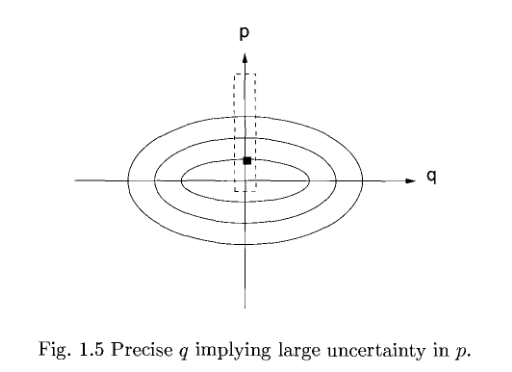
\includegraphics[width=90mm]{muller-kirsten-uncertainty.png}
\end{center}
(Similar pictures can be found in many physics books. This one is from M\"uller-Kirsten's ``Introduction to Quantum mechanics")
\end{frame}

\begin{frame}{Definition of $\Rl^d_\theta$}
    $\Rl^d_\theta$ is a space in the sense of noncommutative geometry: we do not define it directly, but instead
    we define it in terms of its function spaces $L_{\infty}(\Rl^d_\theta),$ $L_2(\Rl^d_\theta),$ $\Sc(\Rl^d_\theta),$ etc.\pause
    The following definition is expedient:
    \begin{definition}
        For $t \in \Rl^d,$ let $\lambda_\theta(t)$ be the unitary operator on $L_2(\Rl^d)$ given by
        \[
            \lambda_\theta(t)u(s) := e^{i(t,s)}u(s-\frac12 \theta t),\quad u\in L_2(\Rl^d).
        \]
        The von Neumann subalgebra of $\Bc(L_2(\Rl^d))$ generated by $\{\lambda_\theta(t)\}_{t\in \Rl^d}$ is denoted $L_{\infty}(\Rl^d_\theta).$
    \end{definition}
\end{frame}

\begin{frame}{Remarks on the definition}
    \begin{enumerate}
        \item{} Note that if $\theta=0,$ this reduces to the description of $L_{\infty}(\Rl^d)$ represented as bounded multipliers on $L_2(\Rl^d),$ and $\lambda_0$ is the operator of pointwise multiplication by the exponential function $s\mapsto \exp(i(t,s)).$
        \item{} A simple computation shows that
        \[
            \lambda_\theta(t+s) = \exp(\frac12 i(t,\theta s))\lambda_\theta(t)\lambda_\theta(s),\quad t,s\in \Rl^d.
        \]
        This is the Weyl form of the canonical commutation relations. It is also a twisted unitary representation of the group $\Rl^d$ by a $2$-cocycle.
        \item{} Heuristically, we have
        \[
            \lambda_\theta(t) = \exp(it_1x_1+\cdots+it_dx_d)
        \]
        where
        \[
            [x_j,x_k] = i\theta_{j,k}.
        \]
    \end{enumerate}
\end{frame}

\begin{frame}{Identification of $L_{\infty}(\Rl^d_\theta)$}
    As a von Neumann algebra, $L_{\infty}(\Rl^d_\theta)$ is not very complicated: it has type $I.$
    \begin{theorem}[Stone-von Neumann]
        There is a $*$-algebra isomorphism
        \[
            L_{\infty}(\Rl^d_\theta) \approx L_{\infty}(\Rl^{\mathrm{\ker(\theta)}})\otimes \Bc(L_2(\Rl^{\frac{\mathrm{rank}(\theta)}{2}})).
        \]
    \end{theorem}
    When $\theta = \begin{pmatrix} 0 & -1 \\ 1 & 0\end{pmatrix},$ this is recognisable as the Schr\"odinger representation;
    \[
        x_1 = M_x,\quad x_2 = -i\partial_x,\text{ on } L_2(\Rl_x).
    \]
\end{frame}

\begin{frame}{Derivatives}
    There is a group action of $\Rl^d$ on $L_\infty(\Rl^d_\theta)$ given on the generators by
    \[
        T_{t}\lambda_\theta(s) = e^{i(t,s)}\lambda_\theta(s),\quad t,s\in \Rl^d.
    \]
    This is the action of \emph{translation}. Say that $x \in L_{\infty}(\Rl^d_\theta)$ is uniformly smooth if
    \[
        t\mapsto T_tx,\quad \Rl^d\to L_{\infty}(\Rl^d_\theta)
    \]
    is smooth. We can define the derivatives
    \[
        \partial_jx := \frac{d}{dt} T_{te_j}(x)|_{t=0}.
    \]
\end{frame}

\begin{frame}{Weyl transform}
    Given $f \in \Sc(\Rl^d),$ let
    \[
        \lambda_\theta(f) = \int_{\Rl^d} f(t)\lambda_\theta(t)\,dt.
    \]
    The space $\Sc(\Rl^d_\theta)$ is defined as the image $\lambda_\theta(\Sc(\Rl^d)).$ This is a $*$-algebra, multiplication is given by twisted convolution
    \[
        \lambda_\theta(f)\lambda_\theta(g) = \lambda_\theta(f\ast_\theta g).
    \]
\end{frame}

\begin{frame}{Noncommutative integral}
    The noncommutative integral $\tau_\theta$ is defined on $\Sc(\Rl^d_\theta)$ by
    \[
        \tau_\theta(\lambda_\theta(f)) := (2\pi)^d f(0).
    \]
    \begin{theorem}
        $\tau_\theta$ extends to a semifinite normal trace on $L_{\infty}(\Rl^d_\theta),$ giving the pair $(L_{\infty}(\Rl^d_\theta),\tau_\theta)$ the structure of a semifinite von Neumann algebra.
    \end{theorem}
    We can therefore define $L_p$ spaces, $L_p(L_{\infty}(\Rl^d_\theta),\tau_\theta),$ which we abbreviate as $L_p(\Rl^d_\theta).$
\end{frame}

\begin{frame}{Harmonic analysis questions}
    Many authors (such as G.~Hong) and most recently M. Ruzhansky and S. Shaimardan and K. Tulenov have addressed the problem of Fourier multipliers on $\Rl^d_\theta.$ I.e., the boundedness of operators
    \[
        m(-i\partial_1,-i\partial_2,\ldots,-i\partial_d):L_p(\Rl^d_\theta)\to L_{q}(\Rl^d_\theta).
    \]
    In terms of $\lambda_\theta,$ we have
    \[
        m(-i\nabla)\lambda_\theta(f) = \lambda_\theta(mf) = (2\pi)^{-d}\int_{\mathbb{R}^d} m(\xi)\lambda_\theta(\xi)f(\xi)\,d\xi.
    \]
%     and associated questions such as Sobolev embedding and elliptic regularity.\pause

    We can also define Sobolev spaces $W^s_p(\Rl^d_\theta)$ (Gonz\'alez-P\'erez, Junge, Parcet) and Besov spaces $B^s_{p,q}(\Rl^d_\theta)$ (Lafleche). Triebel spaces $F^s_{p,q}(\Rl^d_\theta)$ are more challenging.
\end{frame}

\section{PDE on quantum Euclidean spaces}\label{pde_section}

\begin{frame}
    \Huge{Section \ref{pde_section}: PDE on quantum Euclidean spaces}
\end{frame}

\begin{frame}{Linear PDE, constant coefficients}
    Linear PDE with constant coefficients
    \[
        P(-i\nabla)u = f
    \]
    are best studied with Fourier multipliers. Here, things are mostly similar to the commutative case.
\end{frame}

\begin{frame}{Linear PDE, variable coefficients}
    There is a theory (Gonz\'{a}lez-P\'{e}rez, Junge, Parcet [GJP]) of elliptic PDE defined in terms of \emph{left} multipliers:
    \[
        \sum_{|\alpha|\leq m} a_{\alpha} \cdot \partial^{\alpha}u = f
    \]
    where $a_{\alpha}\in C^\infty(\Rl^d_\theta).$

    \pause To analyse these, they defined \emph{left} pseudodifferential operators on $u\in \Sc(\Rl^d_\theta)$ by
    \[
        T_{\sigma}u = (2\pi)^{-d}\int_{\Rl^d} \sigma(\xi)\lambda_\theta(\xi)\tau_\theta(\lambda_\theta(\xi)^*u)\,d\xi.
    \]
    Here, $\sigma:\Rl^d\to L_{\infty}(\Rl^d_\theta)$ is a smooth function satisfying
    \[
        \|\partial_{\xi}^{\alpha}\partial^\beta \sigma(\xi)\|_{\infty} \lesssim (1+|\xi|)^{m-\rho|\alpha|+\delta |\beta|}.
    \]
    \pause
    Using these operators, [GJP] analysed the $L_p$-theory of linear elliptic equations.
\end{frame}

\begin{frame}{Unaddressed question: two-sided linear PDE}
    A trivial modification of [GJP] allows to study \emph{right} PDE
    \[
        \sum_{|\alpha|\leq m} (\partial^{\alpha}u)a_{\alpha} = f
    \]
    where $a_{\alpha}\in C^\infty(\Rl^d_\theta).$

    Something that no-one has addressed (to my knowledge) is the question of two-sided linear PDE, something like
    \[
        \sum_{|\alpha|\leq m} a_{\alpha}(\partial^{\alpha}u)b_{\alpha} = f.
    \]
    This is a new phenomenon in the noncommutative case.\pause
    To analyse it, we would need some kind of theory of \emph{bilateral pseudodifferential operators}.
\end{frame}

\section{Towards a theory of bilateral pseudodifferential operators}\label{towards_section}

\begin{frame}
    \Huge{Section \ref{towards_section}: Towards a theory of bilateral pseudodifferential operators}
\end{frame}

\begin{frame}{Noncommutative Meyer decomposition?}
    If we want to study nonlinear PDE, we need to consider Nemytskij operators
    \[
        u\mapsto F(u)
    \]
    where now $F(u)$ is defined for an operator $u$ using functional calculus. Can we do something similar to Meyer's decomposition?
    \pause
    Answer: Yes, but we need pseudodifferential operators formed out of both left and right multipliers.
\end{frame}

\begin{frame}{Simple case of a noncommutative Meyer decomposition}
    Consider the case $F(u) = u^2.$ Then
    \[
        F(u) = \sum_{j=0}^\infty F(S_{j}u)-F(S_{j-1}u) = \sum_{j=0}^\infty S_{j-1}u \Delta_j u + \Delta_j u S_j u.
    \]
    So the Meyer operator should be the following:
    \[
        m(F,u)v = \sum_{j=0}^\infty S_{j-1}u\Delta_j v+\Delta_j v S_{j}u.
    \]
    Note that here we need both \emph{left} and \emph{right} multiplication. The situation for more general functions $F$ is similar.
\end{frame}

\begin{frame}{Bilateral multiplication}
The algebra $L_\infty(\Rl^d_\theta)^\op$ is the opposite algebra. Given $A \in L_\infty(\Rl^d_\theta)\otimes L_\infty(\Rl^d_\theta)^{\mathrm{op}}$
and $u \in L_\infty(\Rl^d_\theta)$, denote $A\dmult u$ for the linear extension of the mapping $(a\otimes b)\dmult u = aub$.
The Haagerup tensor product $L_\infty(\Rl^d_\theta)\otimes_h L_\infty(\Rl^d_\theta)$ has the property that $\dmult$ has a continuous extension
\[
    \dmult:(L_{\infty}(\Rl^d_\theta)\otimes_{h} L_{\infty}(\Rl^d_\theta)^{\op})\times L_{\infty}(\Rl^d_\theta)\to L_{\infty}(\Rl^d_\theta).
\]
\end{frame}

\begin{frame}{Proposed double symbol definition}
\begin{definition}
    Let $\rho,\delta_1,\delta_2 \in [0,1]$ and $m \in \Rl$. A \emph{bisymbol} in the class $S^m_{\rho,\delta_1,\delta_2}(\Rl^d\times \Rl^d_\theta)$
    is a function:
    \begin{equation*}
        \sigma:\Rl^d\to L_\infty(\Rl^d_\theta)\otimes_h L_\infty(\Rl^d_\theta)^\op.
    \end{equation*}
    Such that for all multi-indices $\alpha,\beta_1,\beta_2\in \Ntrl^d$ we have:
    \begin{equation*}
        \|\partial_\xi^\alpha (\partial^{\beta_1}\otimes \partial^{\beta_2})\sigma(\xi)\|_{L_\infty(\Rl^d_\theta)\otimes_h L_\infty(\Rl^d_\theta)} \leq C_{\alpha,\beta_1,\beta_2}(1+|\xi|)^{m-\rho|\alpha|+\delta_1|\beta_1|+\delta_2|\beta_2|}
    \end{equation*}
\end{definition}
\end{frame}

\begin{frame}{Bilateral pseudodifferential operators}
Let $\sigma\in S^m_{\rho,\delta_1,\delta_2}(\Rl^d\times \Rl^d_\theta).$ Define an operator $T_{\sigma}$ on $u\in \Sc(\Rl^d_\theta)$ by
\begin{equation*}
    T_\sigma u := (2\pi)^{-d}\int_{\Rl^d} (\sigma(\xi)\dmult \lambda_\theta(\xi))\tau_\theta(\lambda_\theta(\xi)^*u)\,d\xi
\end{equation*}
Denote the space of such operators by $\Psi^{m}_{\rho,\delta_1,\delta_2}(\Rl^d_\theta).$
\pause
\begin{conjecture}
\begin{itemize}
    \item{} For $\delta_1+\delta_2<\rho,$ $\Psi^m_{\rho,\delta_1,\delta_2}(\Rl^d_\theta)$ has similar properties of adjointability, composition and asymptotic convergence to traditional pseudodifferential operators. \pause
    \item{} For $\rho=1>\delta_1+\delta_2,$ and $m=0,$ we have boundedness on $L_p(\Rl^d_\theta)$ for $1<p<\infty.$\pause
    \item{} In general for $m=0,$ we have boundedness on $W^s_p(\Rl^d_\theta)$ for $s>0.$
\end{itemize}
\end{conjecture}
\end{frame}

\begin{frame}{Why is it interesting?}
\begin{itemize}
    \item{} If the conjecture is correct, we would have a \emph{genuinely noncommutative} theory of pseudodifferential operators which would allow us to study bilateral PDE and also nonlinear PDE
    over $\Rl^d_\theta.$\pause
    \item{} Following the standard commutative proofs does not seem to work, it seems that new ideas are needed.
\end{itemize}
\end{frame}


\begin{frame}
\structure{\begin{center}
{\Huge{}Thank you for listening!}
\par\end{center}}
\end{frame}


\begin{frame}{Further reading}
\tiny{
    For more about the Meyer decomposition:
    \begin{itemize}
        \item{} M.~Taylor. Partial differential equations III. Nonlinear equations. Second Edition. \textit{Applied Mathematical Sciences} \textbf{117}, Springer, New York, 2011.
        \item{} H.~Bahouri, J.~Chemin, R.~Danchin. Fourier analysis and nonlinear partial differential equations. \textit{Grundlehren der Mathematischen Wissenschaften} \textbf{343}, Springer, Heidelberg, 2011.
        \item{} T.~Runst, W.~Sickel. {Sobolev spaces of fractional order, {N}emytskij operators, and nonlinear partial differential equations}, \textit{De Gruyter Series in Nonlinear Analysis and Applications}, \textbf{3}, {Walter de Gruyter \& Co., Berlin}, {1996}.
    \end{itemize}
    For more about quantum Euclidean spaces, see
    \begin{itemize}
        \item{} S.~Lord, E.~M., F.~Sukochev, D.~Zanin. {Singular traces. {V}ol. 2. {T}race formulas}. \textit{De Gruyter Studies in Mathematics} \textbf{46/2}, De Gruyter, Berlin, 2023.
        \item{} L.~Lafleche. \textit{{On {Q}uantum {S}obolev {I}nequalities},} {\color{red}\href{https://arxiv.org/abs/2210.03013}{arXiv:2210.03013}}.
        \item{} A.~Gonz\'{a}lez-P\'{e}rez, M.~Junge, J.~Parcet. \textit{Singular integrals in quantum {E}uclidean spaces}, {Mem. Amer. Math. Soc.}, \textbf{272}, {2021}.
        \item{} E.~M., F.~Sukochev, X.~Xiong. \textit{Quantum differentiability---the analytical perspective}, {Proc. Sympos. Pure Math.}, \textbf{105}, 2023.
    \end{itemize}
    For more about PDE on quantum Euclidean spaces, see
    \begin{itemize}
        \item{} E.~M. \textit{Nonlinear partial differential equations on noncommutative {E}uclidean spaces}, {J. Evol. Equ.}, \textbf{24}, {2024},
        \item{} M.~Ruzhansky, S.~Shaimardan, K.~Tulenov. \textit{Sobolev inequality and its applications to nonlinear PDE on noncommutative Euclidean spaces}, {\color{red}\href{https://arxiv.org/abs/2408.09100}{arXiv:2408.09100}}.
        \item{} C.~Arhancet, L.~Hagedorn, C.~Kriegler, P.~Portal. \textit{The harmonic oscillator on the Moyal-Groenwald plane: an approach via Lie groups and twisted Weyl tuples}, {\color{red}\href{https://arxiv.org/abs/2312.06143}{arXiv:2312.06143}}.
    \end{itemize}
}
\end{frame}

\end{document}

